%        File: !comp!expand("%:p:t")!comp!
%     Created: !comp!strftime("%a %b %d %I:00 %p %Y ").substitute(strftime('%Z'), '\<\(\w\)\(\w*\)\>\(\W\|$\)', '\1', 'g')!comp!
% Last Change: !comp!strftime("%a %b %d %I:00 %p %Y ").substitute(strftime('%Z'), '\<\(\w\)\(\w*\)\>\(\W\|$\)', '\1', 'g')!comp!
%
\documentclass[a4paper]{article}
\usepackage[catalan]{babel}
\usepackage[utf8]{inputenc}
\usepackage[obeyspaces]{url}
\usepackage{comment}
\usepackage{hyperref}
\usepackage[pdftex]{graphicx}
\begin{document}
\title{Eines per a l'administració remota de servidors}
\maketitle

\begin{comment}
oddsidemargin \the\oddsidemargin \newline
textwidth \the\textwidth \newline
marginparsep \the\marginparsep \newline
marginparwidth \the\marginparwidth \newline
hoffset \the\hoffset \newline
paperwidth \the\paperwidth 
\end{comment}

\section{Synctool}
La missió principal d'aquesta eina \'es la de sincronitzar fitxers de configuració d'un conjunt de servidors remots en base a un repositori local.
A l'igual que pssh utilitza eines com ssh o rsync per a la distribució dels fitxers que s'han de sincronitzar. Un cop sincronitzats en els servidors, synctool permet executar comandes del tipus \verb+service dimoni restart+. Pots, a m\'es, customitzar synctool per a executar m\'es comandes\footnote{\textbf{node} \'es un host dintre d'un grup de computadores o \textbf{cluster}.}.

Per treballar amb synctool hem de fer-ho per ssh sense password. O sigui, del node mestre fins als nodes del clúster ha d'haver autenticació per claus assimètriques. D'igual manera, si volem protegir les claus privades haurem de fer servir l'ssh-agent.


\section{Puppet}
% REFERENCIES %%%%%%%%%%%%%%%%
% http://stackoverflow.com/questions/tagged/puppet
% http://serverfault.com/questions/tagged/puppet
% https://forge.puppetlabs.com/
% https://docs.puppet.com/pe/2015.3/quick_start.html

% què es pot fer amb puppet:
% managing upgrades of hundred debian servers
% Register a new domain/hostname with linux
% Install packaegs using apt-et
% Copy files
% Run some bash scripts
% Generating / managing config files for hosted application
% Execute commands on multiple servers

% TODO crear mòduls de puppet. En forge.puppetlabs.com hi ha un apartat 

\subsection{Instal·lació}
Ens hem de baixar la versió depenent de la nostra distribució:
\begin{verbatim}
root@master:~# wget https://apt.puppetlabs.com/puppetlabs-release-jessie.deb
root@master:~# dpkg -i puppetlabs-release-jessie.deb
\end{verbatim}
La instal·lació del paquet que ens hem baixat ens configura nous repositoris on finalment estàn allotjats els binaris i el codi font de puppet.
\begin{verbatim}
root@master:/etc/apt/sources.list.d# apt-get install puppetmaster
\end{verbatim}
Al final, a part de depèndencies requerides:
\begin{verbatim}
root@master:/etc/apt/sources.list.d# dpkg -l | grep puppet
ii  puppet-common          3.7.2-4   all   configuration management system
ii  puppetlabs-release     1.0-11    all   ``Package to install Puppet ...''
ii  puppetmaster           3.7.2-4   all   configuration management, master service
ii  puppetmaster-common    3.7.2-4   all   configuration management, master common files
\end{verbatim}
Pel client fem el mateix procès però en comptes d'instal·lar el paquet \verb+puppetmaster+ instal·lem \verb+puppet+. Despr\'es configurem el fitxer \verb+/etc/hosts+ pròpiament per a que tots dos es vegin per el nom de la màquina.

\subsection{Hello World}
Hem de crear un fitxer sota de \verb+/etc/puppet/manifiest+ amb extensió \verb+.pp+. Aquest fitxer \'es un fitxer de codi declaratiu de puppet on definim els nostres recursos. Cada recurs \'es d'un tipus determinat i t\'e un nom. Això \'es el mínim que ha de tenir. Veurem que pot tenir propietats amb valors (parell de claus separades per \verb+=>+). El codi t\'e la següent aparença:
\begin{verbatim}
notify{'Hello world':
}
\end{verbatim}
Aquest \'es un recurs de tipus \textit{notify} Ara el que hem de fer \'es executar-lo:
\begin{verbatim}
$ puppet apply hello.pp
Notice: Compiled catalog for master.home in environment production in 0.05 seconds
Notice: Hello world
Notice: /Stage[main]/Main/Notify[Hello world]/message: defined 'message' as 'Hello world'
Notice: Finished catalog run in 0.04 seconds
\end{verbatim}
Un altra tipus de recurs \'es \textit{file} el qual serveix per crear un fitxer amb un determinat contingut. En aquest exemple anem a crear un fitxer a \verb+/tmp+ que es diu \textit{demo.txt}. El fitxer s'ha de crear si no existeix i el seu contingut ha de ser 'Hello World':
\begin{verbatim}
usuario@master:/etc/puppet/manifests$ cat demo.pp 
file {'/tmp/demo.txt':
    # si el fitxer no exixteix, que el crei
    ensure => present,
    # contingut del fitxer
    content => 'Hello World',
}
usuario@master:/etc/puppet/manifests$ puppet apply demo.pp 
Notice: Compiled catalog for master.home in environment production in 0.21 seconds
Notice: Finished catalog run in 0.03 seconds
usuario@master:/etc/puppet/manifests$ ls /tmp
demo.txt
usuario@master:/etc/puppet/manifests$ cat /tmp/demo.txt 
Hello Worldusuario@master:/etc/puppet/manifests$ 
\end{verbatim}

\subsection{Test Model Client-Servidor}
Anem a fer que un agent apliqui un .pp del servidor. Per defecte, el .pp s'ha de dir \textit{site.pp}. És el manifest per defecte que els clients llegeixen del master server. En arrancar l'agent, si tot va b\'e el procès \'es el següent (el primer cop que s'executa l'agent s'estableixen els certificats):
\begin{itemize}
	\item Agent genera claus i envia al màster la seva clau pública.
	\item Master li torna la clau signada i la torna al client. Ho farem a mà.
	\item Agent es baixa .pp i executa la configuració
\end{itemize}

\begin{verbatim}
root@client0:~# puppet agent --server master.home --verbose --no-daemonize 
														 --waitforcert 10
Info: Creating a new SSL key for client0.home
Info: csr_attributes file loading from /etc/puppet/csr_attributes.yaml

Info: Certificate Request fingerprint (SHA256): 
  6D:AD:C0:57:4E:82:67:79:0F:25:35:39:CF:C1:35:67:ED:12:6C:27:32:87:43:E1:...
Notice: Did not receive certificate
Notice: Did not receive certificate
Notice: Did not receive certificate
Notice: Did not receive certificate
Notice: Did not receive certificate
Notice: Did not receive certificate
Info: Caching certificate for client0.home
Notice: Starting Puppet client version 3.7.2
Info: Retrieving pluginfacts
Info: Retrieving plugin
Info: Caching catalog for client0.home
Info: Applying configuration version '1457863005'
Notice: /Stage[main]/Main/File[/tmp/demo2.txt]/ensure: created
Notice: Finished catalog run in 0.12 seconds
^CNotice: Caught INT; calling stop
root@client0:~# ls /tmp
demo2.txt
root@client0:~# 
\end{verbatim}
En el master hem de tenir el \textit{site.pp}:
\begin{verbatim}
file {'/tmp/demo2.txt':
  # si el fitxer no exixteix, que el crei
  ensure => present,
  # contingut del fitxer
  content => 'Hello World',
  owner => 'root',
  mode => 777,
}
\end{verbatim}
En el client, l'avís \verb+Notice: Did not receive certificate+ vol dir que no ha rebut el seu certificat signat per el master. Per fer-ho, des del master:
\begin{verbatim}
root@master:/etc/puppet/manifests# puppet cert sign client0.home
\end{verbatim}
Per veure els certificats dels clients:
\begin{verbatim}
root@master:/etc/puppet/manifests# puppet cert list
\end{verbatim}
Al final, en aquest exemple, se'ns haurà creat un fitxer a tmp amb propietari i permisos com els configurats en el \textit{site.pp}.

\paragraph{Problemes}\\
\begin{enumerate}
	\item que no coincideixin els noms de les màquines amb els noms que s'han posat en els certificats. Podem tocar el paràmetre certname a la configuració del master, o afegir en el \verb+/etc/hosts+ com a nom a les màquines el que hem posat en el certificat i en la comanda de l'agent, 
		\begin{verbatim}
		--server <posem el nom que surt al certificat>
		\end{verbatim}
	\item que no s'envii el certificat des de l'agent. Tornem a començar: des del master, esborrem el certificat de l'agent i, des del client, igual:
	\begin{itemize}
		\item Master:
			\begin{verbatim}
			root@master:/etc/puppet/manifests# puppet cert clean client0.home
			\end{verbatim}
		\item client:
			\begin{verbatim}
			root@client0:~# find /var/lib/puppet/ssl -name client0.home.pem -delete
			\end{verbatim}
			I tornem a executar la comanda en l'agent.
			% NOTA: TINC IMATGES Fetes
	\end{itemize}
	\item en el client, l'agent no s'arrenca donant un error. Amb això, hem de tenir clar les següents coses:
		\begin{enumerate}
			\item En instal·lar \textit{puppet} en el client tenim un servei \textit{puppet agent} iniciat per defecte.
			\item Si hi ha un \textit{agent puppet} iniciat no es pot iniciar cap altre, per la qual cosa, hem de parar el que hi hagi arrancat i hem de treure el bloqueig de que s'inicii qualsevol agent amb la comanda \verb+puppet agent --enable+
			\item Un cop desbloquejat, ja podem executar la comanda per rebre la configuració del master.
		\end{enumerate}
\end{enumerate}

\subsection{Nodes}
Els nodes permeten a un servidor \textit{Puppet} tenir diferents recursos diferenciats per clients. Els nodes es defineixen en el manifest \textit{site.pp}. Exemple del fitxer \textit{site.pp}:

\begin{verbatim}
# el nom que li donem al node correspon al nom de la màquina
node client0 {
  package {'nginx':
    # ens hem d'assegurar que el paquet estigui instal·lat
    # si no ho està, s'instal·la
    ensure => installed,
  }  	
}

# nodes no definits explícitament
node default {
  notify {'Default node':
  }
}
\end{verbatim}
Agent \textit{client0}, aleshores, en recuperar la configuració, haurà instal·lat \textit{nginx} (abans no hi era):
\begin{verbatim}
root@client0:/home/usuario# puppet agent --server master.home --verbose 
                                         --no-daemonize --waitforcert 10
Notice: Starting Puppet client version 3.7.2
Info: Retrieving pluginfacts
Info: Retrieving plugin
Info: Caching catalog for client0.home
Info: Applying configuration version '1458290609'
Notice: /Stage[main]/Main/Node[client0]/Package[nginx]/ensure: 
                          ensure changed 'purged' to 'present'
Notice: Finished catalog run in 60.09 seconds
^CNotice: Caught INT; calling stop
root@client0:/home/usuario# dpkg -l nginx
ii  nginx          1.6.2-5+deb8 all          small, powerful, scalable web/prox
\end{verbatim}
Si a la propietat \textit{ensure} li donem el valor \textit{absent}, succeirà el contrari.
\subsection{Recursos}
\begin{itemize}
	\item \textbf{notify}
	\item \textbf{file}
	\item \textbf{package}: defineix un paquet de software a instal·lar o desinstal·lar en un node.
	\item \textbf{service}: Possibles propietats:
		\begin{itemize}
			\item \verb+ensure+, que pot prendre els valors \textit{stopped} o \textit{running}
			\item \verb+enable+, per configurar el seu arranc automátic, que pot prendre els valors \textit{true} o \textit{false}.
			\item \textit{require}. Si volem fer esmena d'una altre recurs. Veure la següent subsecció sobre dependències de recursos del recurs \textit{service}
		\end{itemize}
	\item \textbf{exec}: per executar comandes.
	\item \textbf{group}: gestionar grups \textit{Unix like}.
	\item \textbf{user}: gestionar usuaris \textit{Unix like}.
\end{itemize}
\subsection{Dependències entre recursos en el recurs \textit{service}}
Si tenim un recurs de tipus \textit{service} el que volem, per exemple, \'es que estigui iniciat però sempre i quan tinguem el paquet instal·lat, o que es notifiqui cada canvi en el fitxer de configuració d'aquest servei ja que no es reflectiràn aquests canvis si no es fa, com a mínim, un \textit{reload} del servei.

Qualsevol crida que fem a un recurs des d'un altre recurs, com a regla de sitaxi, hem de començar a nomenar el tipus de recurs amb lletra majúscula i, com si fos un array, entre corxets i cometes, especificar el nom del recurs al que fem referència:

\scalebox{.5}{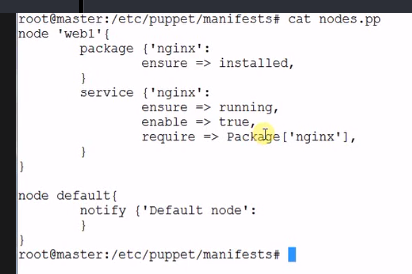
\includegraphics{dependencies.png}}
\subsection{Modulització: Classes i definició de recursos}
Els mòduls es creen sota el directori \verb+/etc/puppet/modules+. Cada mòdul es crea sota un directori dintre del directori modules i la seva estructura bàsica porta els següents directoris: \verb+manifests+, \verb+files+ i \verb+templates+. Al directori \verb+manifests+ hi ha d'haver un fitxer que \'es el que s'executa primer quan es fa referència a un mòdul, \verb+init.pp+. Per incloure un mòdul en el catàlog d'un node:\\

\scalebox{.5}{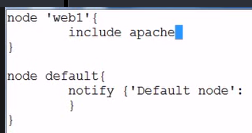
\includegraphics{include.png}}\\
El directori \textit{files} serveix per contenir els fitxers de configuració dels serveis, etc.

La diferència entre classes i definicions \'es que les classes les inclouem en els llocs on les volem fer servir i les definicions simplement les cridem. Vindria a ser com la diferència entre \textit{includes} i \textit{funcions} en un llenguatge estructurat.
\subsubsection{Classes}
Les classes venen a ser com includes. Són blocs de codi \textit{puppet}. No afegeixen cap recurs al catàlog de cap node. Per a que sí formin part d'un catàlog, han de ser declarades. Poden contenir subclasses, les quals es criden amb ::. Exemple de classe:
\begin{verbatim}
#dintre de class definim els nostres recursos:
class base{
  file {‘/etc/passwd’:
    owner => ‘root’,
    group => ‘root’,
    mode => ‘0644’,
  }
  file {‘/etc/shadow’:
    owner => ‘root’,
    group => ‘root’,
    mode => ‘0440’,
  }
}
\end{verbatim}
Un altre exemple de classe que, a m\'es, t\'e depend\'encies:\\

\begin{figure}[h]
	\centering
	\scalebox{.5}{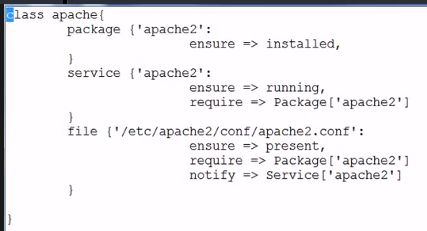
\includegraphics{class_depend.png}}\\ 
\end{figure}
%\scalebox{.5}{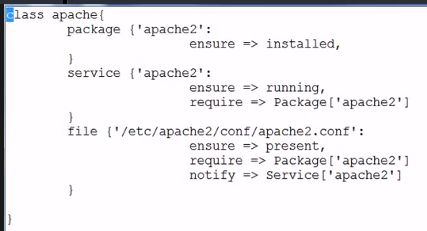
\includegraphics{class_depend.png}}\\ 

\paragraph{Subclasses\\}
Com es pot resoldre el problema de les dependències amb subclasses? Podem crear, en el mateix directori on hem creat el fitxer \textit{init.pp} al mòdul apache (\verb+/etc/puppet/modules/apache/manifests+) el fitxer \textit{install.pp} per definir la subclasse \textit{install} que representa el recurs package:
\begin{verbatim}
class apache::install {
  package {
    ensure => installed,
  }
}
\end{verbatim}
I, de la mateixa manera, el fitxer \textit{service.pp} i \textit{config.pp}:
\begin{figure}[hb]
	\scalebox{.4}{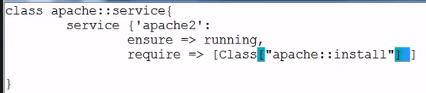
\includegraphics{subclass_service.png}}
	\scalebox{.4}{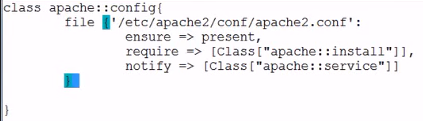
\includegraphics{subclass_config.png}}\\ 
	\scalebox{.7}{Fixar-se que quan fem referència a un element, un recurs, una classe, etc, ho fem amb la primera lletra en majúscules.}\\ 
\end{figure}
\begin{figure}[h]
	\centering
	%\scalebox{.7}{Referenciem en la classe principal de la següent manera:}
	\scalebox{.5}{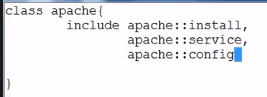
\includegraphics{class_final.png}}\\ 
	\scalebox{.7}{Exemple obsolet. S'han de treure les comes i potser cal ficar \textit{include} en les tres línies}
\end{figure}
\subsubsection{Definitions}
A diferència de les classes, una vegada creada una definició, ja actua com un tipus de recurs. Es pot parametritzar i \'es avaluada cada vegada en funció d'aquests paràmetres.

Anem a veure un exemple seguint l'exemple d'abans del mòdul d'apache. Crearem la definició que serà per fer servir recursos que faràn referència  a virtualhosts. Primer de tot creem el fitxer \textit{vhost.pp} dintre del mateix directori \textit{manifests} on hem creat el fitxer init del módul apache:
\begin{verbatim}
#entre parèntesi declarem els arguments.
#hi han dos arguments que sempre hi són, que són $title i $name.
define apache::vhost($port, $docroot){
  ``/etc/apache2/conf/$name'':
    # fisicament aquest fitxer font haurà d'estar al directory files 
    # dintre del mòdul.
    source => ``puppet:///modules/apache/apache2.conf'',
    owner => ``apache``,
    group => ''apache``,
    mode => 755,
    require => [Class[''apache::install``]],
    notify => [Class[''apache::service``]]
}
\end{verbatim}
Despr\'es la fem servir a \textit{install.pp} d'apache:
\begin{verbatim}
class apache {
  include apache::install,
  include apache::service,
  include apache::config,

  # el primer argument \'es el $name, el nom del recurs.
  # faig servir un recurs de tipus apache\:\:vhost que te per nom apache2.conf
  # t\'e per paràmetres $port i $docroot
  apache::vhost {``apache2.conf'':
    $port => 80,
    $docroot => ``/var/www/html/mysite'',
  }
}
\end{verbatim}
\subsection{Ordre d'avaluació entre els recursos}
Per defecte serà en l'ordre en la que s'han definit aquests recursos. Sinó, es pot control·lar o alterar l'ordre gràcies a les propietats \textit{require} i \textit{before} dintre dels recursos i fent referència (o sigui, donant com a valor d'aquestes propietats) als recursos que li acompanyen.
\subsection{Templates}
Les plantilles es fan servir per crear fitxers amb valors dinàmics que passem als clients o agents. Es creen sota els mòduls, en el directori \textit{templates} i poden fer ús de variables, expressions, llistats, etc. que es calculen en temps d'execució. Les plantilles van dintre dels directoris dels mòduls, en els subdirectoris \textit{templates}. Per fer ús d'un template s'ha de cridar la funció \textit{templates}.
\begin{figure}[h]
	\centering
	\scalebox{.5}{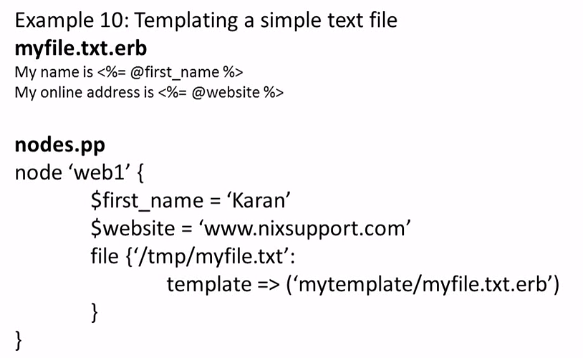
\includegraphics{templates.png}}\\ 
\end{figure}
Anem  veure un exemple de com crear i fer servir plantilles. Anem a crear una classe que es diu \textit{linuxbase} la qual farem servir per definir els recursos de client\_0. Aquesta classe tindrà una subclasse, que \'es a la que cridarà directament, \textit{tmp} que definirà un recurs de tipus file amb un contingut que estarà definit per una plantilla:
\begin{enumerate}
	\item Creem els subdirectoris necessaris a \verb+/etc/puppet/modules+: \verb+linuxbase+, \verb+linuxbase/manifests+ i \verb+linuxbase/templates+.
	\item Definim la plantilla a \verb+linuxbase/templates+. Creen un fitxer que es diu myfile.txt.erb. Les plantilles s'han de crear amb l'extensió \verb+.erb+ (llenguatge \textit{erb}, \textit{ruby standard library}):
		\begin{verbatim}
		my name is <%= @first_name %>
		my website is <%= @website %>
		\end{verbatim}
	\item Fem ús de la plantilla a la subclasse \verb+linuxbase::tmp+. Per això definim la subclasse en \verb+linuxbase/manifests/tmp.pp+:
		\begin{verbatim}
		class linuxbase::tmp{
		  $first_name = ``Juan''
		  $website = ``www.aguileraj.com''
			# la plantilla agafa totes les variables definides en aquest scope
		  file {'/tmp/file.txt':
		    content => template (``linuxbase/myfile.txt.erb''),
		  }
		}
		\end{verbatim}
	\item I ara definim la classe \verb+linuxbase+ que anirà dintre del fitxer \verb+linuxbase/manifests/init.pp+:
		\begin{verbatim}
		class linuxbase {
		  include linuxbase::tmp
		}
		\end{verbatim}
	\item en executar puppet en mode client en client0 s'hauria d'haver creat el fitxer a \verb+/tmp/file.txt+ amb el contingut:
		\begin{verbatim}
		my name is Juan
		my website is www.aguileraj.com
		\end{verbatim}
\end{enumerate}
\subsection{Facts}
Variables predefinides del sistema i amb les quals podem tamb\'e crear estructures de control de fluxe com \textit{if} o \textit{switch} o \textit{if \ldots else}. Per veure la llista de \textit{facts} definides en el sistema, \verb+facter+. Anem a veure un exemple en el que, depenent de la variable d'entorn o \textit{facter} \verb+$osfamily+, instal·lem el paquet \textit{apache2} si el sistema \'es \textit{Debian} o el paquet \textit{httpd} si \'es \textit{Red Hat}. Ho farem com en l'exemple anterior, a \textit{templates}, creant una subclasse de la classe \textit{linuxbase} que es digui \textit{install}. Fitxer \verb+/etc/puppet/modules/linuxbase/manifests/install.pp+:
\begin{verbatim}
class linuxbase::install {
  if $osfamily ==  'Debian' {
    package {'apache2':
      ensure => installed,
    }
  } elsif $osfamily ==  'RedHat' {
    package {'httpd':
      ensure => installed,
    }
  }
}
\end{verbatim}
\subsection{Gestionar usuaris i grups Unix like des de puppet}
Els recursos associats són \textit{group} i \textit{user}. En el següent exemple podem visualitzar les propietats que poden tenir:
\begin{verbatim}
group {'db-admins':
  ensure => present,
	gid => 4002,
}
user {
  uid => 2014,
	home => '/home/karan'
	# si la següent propietat no està a true, 
	# no podrem crear la home o gestionar la 
	# home adecuadament (amb els permisos correctes, per exemple)
  managehome => true,
	gid => 1000,
	shell => '/bin/bash',
	groups => ['db-admins'],
}
\end{verbatim}

\subsection{Com executar comandes Linux amb puppet}
En aquest cas el recurs \'es \textit{exec} les propietats que pot portar:
\begin{figure}[h]
	\centering
	\scalebox{.3}{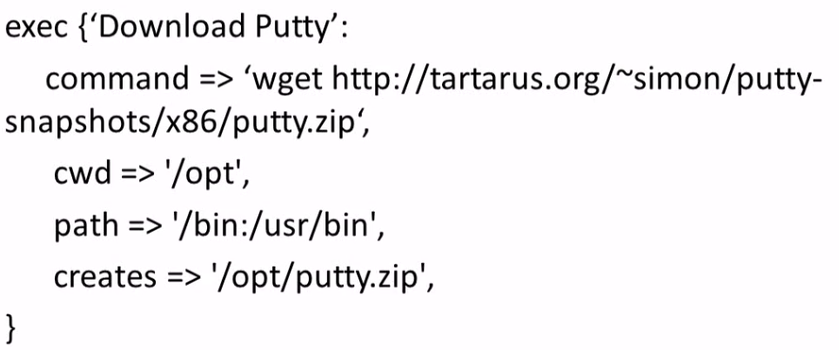
\includegraphics{exec.png}}
\end{figure}
\subsection{Síntesi}
\subsubsection{Instal·lació de Lamp server en un servidor amb puppet}
\paragraph{Instal·lació manual de Lamp en un servidor \\}
\begin{enumerate}
	\item Actualitzar les llistes dels repositoris del sistema
		\begin{verbatim}
		# apt-get update
		\end{verbatim}
	\item Ens instal·lem \textit{apache2}
		\begin{verbatim}
		# apt-get install apache2
		\end{verbatim}
	\item Ara ens instal·lem el paquet \textit{php5}. Instal·la automàticament altres paquets.
		\begin{verbatim}
		# apt-get install php5
		\end{verbatim}
	\item \textit{php5-mysql}. Requereix \textit{php5}. Instal·la automàticament altres paquets.
		\begin{verbatim}
		# apt-get install php5-mysql
		\end{verbatim}
	\item Reiniciem apache2. 
		% en puppet, propietat next? MIrar ordre d'execució.
	\item instal·lem el paquet \textit{mysql-server} i li donem un password a root (\textit{mysql})
	\item Idem amb libmysqlclient-dev. Suposo que serà necessari tenir prèviament mysql-server. % necessari?
\end{enumerate}

% https://forge.puppetlabs.com/puppetlabs/mysql
% https://forge.puppetlabs.com/puppetlabs/apache
% https://forge.puppetlabs.com/puppetlabs/apt
% https://docs.puppetlabs.com/puppet/latest/reference/lang_namespaces.html

\subsection{TODOs}
\scalebox{.5}{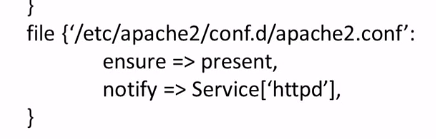
\includegraphics{notify_property.png}}\\
Per exemple, el que fa aquesta propietat \textit{notify} \'es avisar de qualsevol canvi en el fitxer de configuració per a que el servei HTTP reinicii.

\paragraph{Per a què serveix la comanda puppet apply -e '\<comanda\>' \\}
\section{bcfg2}\cite{BCFG2}

\section{Sobre aquest document}
\textbf{Copyright}\copyright\ \textbf{\the\year\ Juan Aguilera}.\\
Permission is granted to copy, distribute and/or modify this document under the terms of the GNU Free Documentation License, Version 1.3 or any later version published by the Free Software Foundation;\\
with no Invariant Sections, no Front-Cover Texts, and no Back-Cover Texts.\\
A copy of the license is included in the section entitled \href{http://www.gnu.org/licenses/fdl.html}{``GNU Free Documentation License``}.

\begin{thebibliography}{99}
	\bibitem{SYNCTOOL} \url{http://walterdejong.github.io/synctool/}
	\bibitem{BCFG2} \url{http://docs.bcfg2.org/index.html}
	\bibitem{COMP_EINES} \url{https://en.wikipedia.org/wiki/Comparison_of_open-source_configuration_management_software}
	\bibitem{PUPPET} \url{https://forge.puppetlabs.com/} 
\end{thebibliography}

\end{document}


